%% LyX 2.0.5.1 created this file.  For more info, see http://www.lyx.org/.
%% Do not edit unless you really know what you are doing.
\documentclass[usenatbib]{article}
\usepackage[latin9]{inputenc}
\usepackage[a4paper]{geometry}
\geometry{verbose}
\usepackage{color}
\usepackage{float}
\usepackage{graphicx}

\makeatletter

%%%%%%%%%%%%%%%%%%%%%%%%%%%%%% LyX specific LaTeX commands.
%% Because html converters don't know tabularnewline
\providecommand{\tabularnewline}{\\}
%% A simple dot to overcome graphicx limitations
\newcommand{\lyxdot}{.}


%%%%%%%%%%%%%%%%%%%%%%%%%%%%%% Textclass specific LaTeX commands.
\usepackage{jcappub}

%%%%%%%%%%%%%%%%%%%%%%%%%%%%%% User specified LaTeX commands.






%%%%%%%%%%%%%%%%%%%%%%%%%%%%%% LyX specific LaTeX commands.
%% A simple dot to overcome graphicx limitations
%Make my life significantly easier
\usepackage[left,modulo]{lineno}
\global\long\def\bd{{\bm{\delta}}}

\makeatother

\begin{document}

\section{Mass Resolution}

In this section, we investigate how mass resolution affects on halo
bias and mass functions. We prepare two samples with $256^{3}$ and
$512^{3}$ particles in the cubic box, whose side length is $256h^{-1}{\rm Mpc}$.
Note that both samples are simulated from the same initial density
field with the same number of time steps.

We first show comparison of cumulative mass functions in Figure \ref{fig:massFn_massResolution}.
We calculate mean and its error through the bootstrap method, generating
100 samples by choosing halos randomly from an output of the simulation.
In the right panel of Figure \ref{fig:massFn_massResolution}, the
mean and its error for the samples of $512^{3}$ particles are indicated
as shaded regions and the mean for $256^{3}$ particles indicated
as ci\textcolor{black}{rcles. The discrepancy in the mass functions
between $256^{3}$ particles and $512^{3}$ particles becomes larger
on large halo masses. This is mainly because there are a few large
halos and therefore it is more sensitive to the differences in the
number of halos. It is possible that samples with higher mass resolutions
resolve more small halos and a multiple halos in the samples with
$512^{3}$ particles correspond to one larger halo in the $256^{3}$-particles
samples. We also see that agreement between the samples of those two
mass resolutions is better at lower redshift, possibly because particles
are more well clustered at lower redshift. Those differences on mass
functions can cause systematic errors on halo bias due to selection
of halos. }

In Figure \ref{fig:haloAuto_mass}, we compare halo-matter cross power
spectra at various redshifts. Here, we use the same matter density
field generated with $256^{3}$ particles for both cases, and we select
halos based on the ``soft mass-cut'' method using the function described
below. 

\begin{equation}
<N_{halo}(M)>=\frac{1}{2}{\rm erfc}(\frac{{\rm log(M_{cut}/}M)}{\sqrt{2}\sigma}),
\end{equation}
where we set ${\rm M_{cut}=10^{13.0}[{\rm M_{\odot}]}}$ and $\sigma=0.5$.
Using the soft mass-cut method, we generate 10 samples to compute
the cross power spectra and their errors. From now on, we use the
same method for halo selections to compute power spectra. Note that
the ratio of those cross power spectra is equivalent to the ratio
of halo bias. Figure \ref{fig:haloAuto_mass} shows the halo bias
for $256^{3}$ particles is smaller than for $512^{3}$ particles
and they agree well within 2\%. This also implies the effect on halo
bias due to different mass resolusion is less sensitive compared to
the effect on mass functions. 

\begin{figure*}
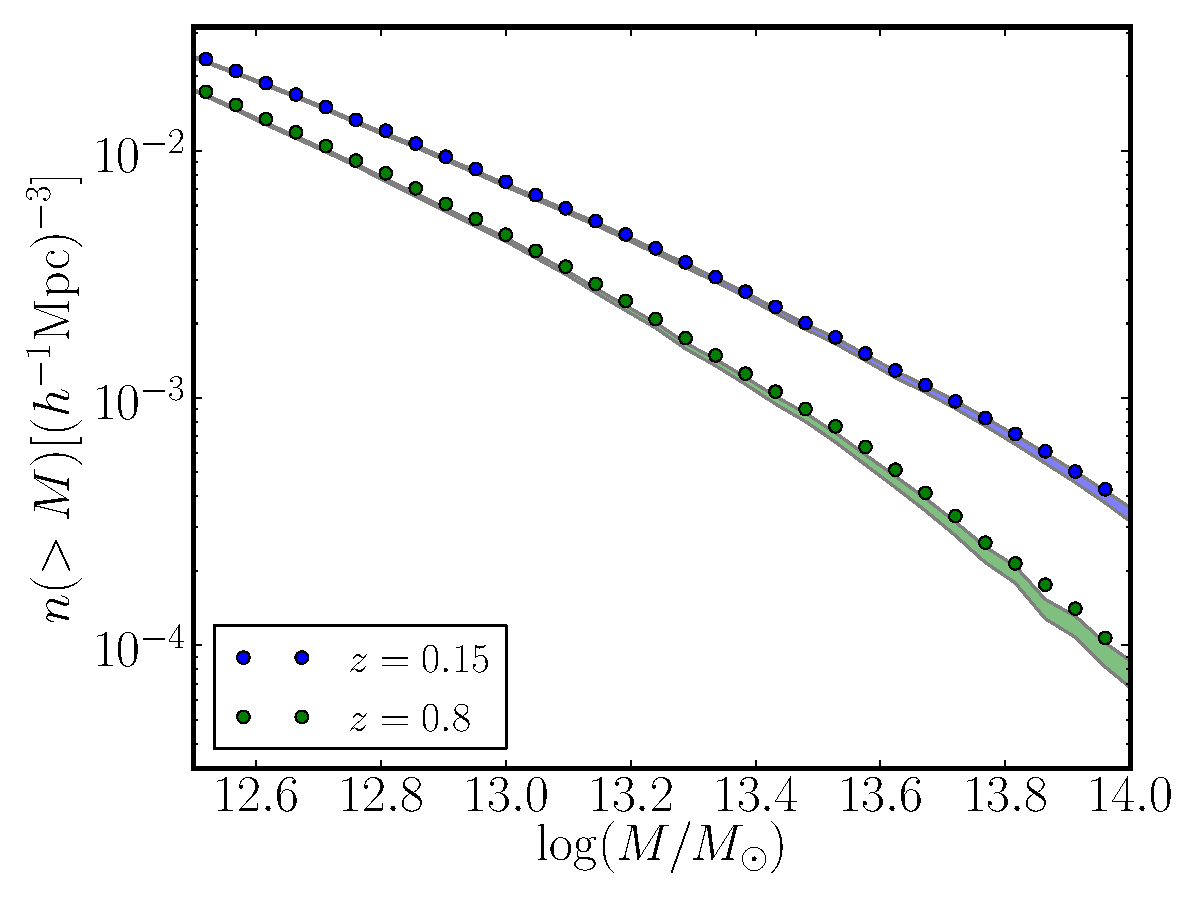
\includegraphics[width=1\columnwidth]{/Users/old_ts485/Dropbox/big-sims/Plots/haloNum_massResolution}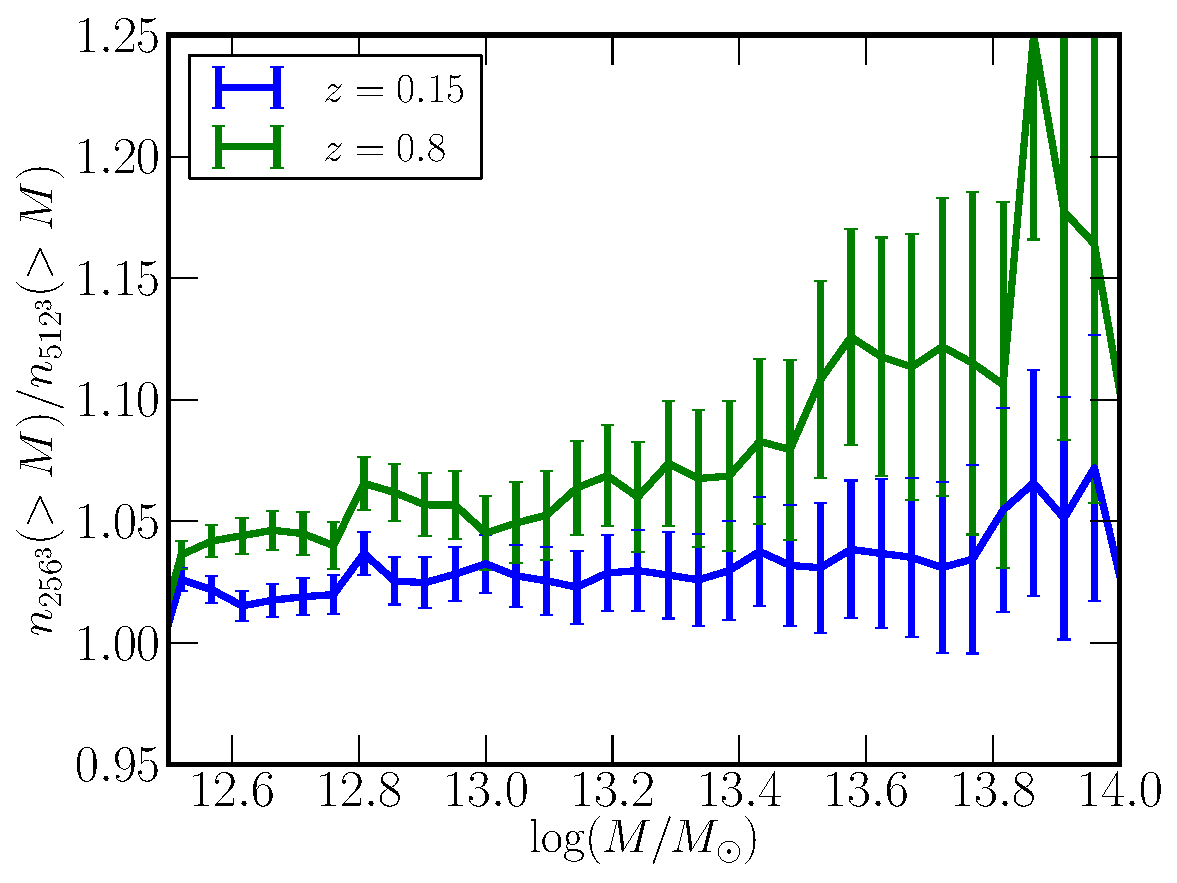
\includegraphics[width=1\columnwidth]{/Users/old_ts485/Dropbox/big-sims/Plots/haloRatioNum_massResolution}

\caption{\label{fig:massFn_massResolution}Left: Cumulative mass functions
for the simulations of $512^{3}$ and $256^{3}$ particles. Shaded
regions are the mean with errors for the samples of $512^{3}$ particles
calculated through the bootstrap method. Circles are the mean for
$256^{3}$ particles. Right: Ratio of cumulative mass functions between
the samples of $512^{3}$ and $256^{3}$ particles. The deviation
from one on large halo masses is mainly caused by the fewer number
of large halos.}
\end{figure*}


\begin{figure}
\includegraphics[width=1\columnwidth]{/Users/old_ts485/Dropbox/big-sims/Plots/crossMatter_massRes_softMcut13\lyxdot 0_s0\lyxdot 5}

\caption{\label{fig:haloAuto_mass}Ratio of halo-matter cross power spectra
between the samples of $512^{3}$ and $256^{3}$ particles for various
redshifts. The overall agreements are all within 2\%. Note that halos
are selected based on the ``soft masscut'' method described in the
section.}
\end{figure}



\section{Selection of the minimal time steps}

The goal in this section is to determine the sufficient time-stepping
scheme to resolve halo positions and masses reliably for the future
galaxy surveys. We are particularly interested in reducing the number
of sub\textcolor{black}{-cycles, because most of computational time
is spent in the short-range time solver. In order to quantitatively
evaluate different time-stepping schemes, we run a set of convergence
tests using smaller simulation boxes. As already explained, our aim
is to carry out simulations in approximate $(4h^{-1}{\rm Gpc})^{3}$
volumes with $4096^{3}$ particles, leading to a particle mass of
\textasciitilde{}$10^{11}{\rm M_{\odot}}$. We scale down these volumes
to $(256h^{-1}{\rm Mpc})^{3}$ with $256^{3}$ particles, which keeps
the particle mass unchanged. In addition, we have carried out one
simulation with $512^{3}$ particles with exactly the same phases
for detailed mass resolution studies. The number of time steps were
chosen as 450/5, 300/3, 300/2, 150/3, 150/2, where the first number
indicates the number of long time steps and the second number the
number of short time steps for each long time step. Note that all
the samples used in this section are at redshift $z=0.15$. After
determining our target time-stepping scheme, we do a more detailed
examination at various redshifts in the next section. To provide some
idea of the variation across all of the choices, we compare observable
quantities including mass functions and power spectra in real and
redshift spaces, as well as masses and positions of halos matched
one by one. Based on a number of convergence tests, the 300/2 combination
turned out to be the best choice.}


\subsection{Observables}

We investigate how mass resolution and the number of time steps affects
the observable quantities including mass functions and power spectra.


\subsubsection{Time Steps}

We first compute mass functions from outputs of different time-stepping
schemes, as shown in Figure \ref{fig:massFn_step}, where we compare
simulations with reduced number of time steps to the 450/5 simulation.
In Figure \ref{fig:massFn_step}, we show the ratio $n(>M)/n_{450/5}(>M)$,
where $n_{450/5}(>M)$ is a cumulative mass function for the 450/5
simulation and $n(>M)$ is a cumulative mass function for different
time steps shown in different colors. Here, we use a fixed linking
length of $b=0.16$ times the mean interparticle separation for all
the simulations to identify halos through the friends-of-friends (hereafter,
fof) algorithm, and halo masses are assigned based on the number of
particles contained in halos. We see that the cumulative mass functions
for 150 global steps have smaller amplitudes overall than those for
450 and 300 global steps. This is because a smaller number of time
steps makes halos more diffused and the fixed linking length cannot
connect some particles in the outputs of 150 global steps whose corresponding
particles are connected in the simulations of larger global steps.
In addition to the difference in global steps, sub-cycles also make
the internal structure of halos more diffused and this leads to the
suppression on the number of low-mass halos. In \textcolor{red}{Manera
et al. 2012} which uses the second-order Lagrangian perturbation theory
to generate dark matter fields, they used a longer linking length
and reassigned halo masses in order to solve the same problem of having
diffused halos. We find that overall agreement between the simulations
of 450/5 and 300 global steps on mass functions is sufficient.

\begin{figure}
\includegraphics[width=1\columnwidth]{/Users/old_ts485/Dropbox/Tomomi/HACC/Conv/Plots4lyx/haloRatioNum256_z0\lyxdot 15}

\caption{\label{fig:massFn_step} Comparison of cumulative mass functions in
different simulations taking the 450/5 as a reference. Lines, from
top to bottom, correspond to different time steps, 300/3 (blue), 300/2
(green), 150/3 (red), and 150/2 (cyan) respectively. As shown, the
agreement between 300 global steps and the 450/5 is close to one on
large halo mass and sub-cycles make differences only on small halo
mass.}
\end{figure}


The next measure of interest is the cross power spectra between halos
and matter densities, as shown in Figure \ref{fig:crossMater_step}.
Figure \ref{fig:crossMater_step} shows the ratio $P_{hm}/P_{hm,450/5}$
at $z=0.15$, where $P_{hm,450/5}$ is the cross power spectrum for
450/5 and $P_{hm}$ is the cross power spectrum for other time steps
labeled in the figure. To calculate the cross power spectra, we use
the output of the 450/5 simulation for the matter densities for all
the halo sample. In this way, the ratio $P_{hm}/P_{hm,450/5}$ is
equivalent to the ratio of halo bias between the 450/5 and other time-steps,
showing systematic errors due to the de-tuned simulations. Here, we
use only one realization for the calculations and this is partly why
our cross power spectra are noisy on large scales. Another contribution
to the noise is the relatively small volume of the simulation box.
We see that the agreement between 450/5 and 300 global steps is remarkably
good and that the differences are well within 5\% on any scales. In
addition, we see the systematic error on halo biases for 150 global
steps is also within 5\% on large scales. This implies that halo bias
on large scales is not largely affected by reduction of the time steps.

\begin{figure}
\includegraphics[width=1\columnwidth]{/Users/old_ts485/Dropbox/Tomomi/HACC/Conv/Matching_halos/20130703/crossMatter_m450_timestep_softMcut13\lyxdot 0_s0\lyxdot 5_z0\lyxdot 15}

\caption{\label{fig:crossMater_step} Ratio of halo-matter cross pow\textcolor{black}{er
spectra as a function of time steps with respect to the 450/5. The
agreements with the 450/5 are all within 5\% on large scales. For
300 global steps, both agree well even on small scales with little
difference by sub-cycles. Note that the halos are selected based on
the soft mass-cut method with $M_{cut}=13.0$ and $\sigma=0.5$.}}
\end{figure}


The final quantitative comparison here is auto power spectra in redshift
space. We are particularly interested in how de-tuning affects the
velocity fields and therefore, the redshift space. The result is shown
in Figure \ref{fig:rsd_step} as the ratio $P_{s}/P_{s,450/5}$, where
$P_{s,450/5}$ is the auto power spectrum calculated from the simulation
of 450/5 and $P_{s}$ is the auto power spectrum with reduced number
of time steps. Before taking the ratio, we subtracted a Poisson shot
noise contribution of $1/n$. We see that the simulations with 150
global steps do not have the same velocity fields as the 450/5 simulation,
because their ratios for the redshift-space power spectra between
450/5 and 150 global steps show larger deviations compared to the
ratios for halo biases, shown in Figure \ref{fig:crossMater_step}.
This implies that the simulations with only 150 global steps have
systematic errors in the measurement of the growth factor through
redshift-space distortions. For 300 global steps, the agreement with
the 450/5 simulation is sufficiently good on large scales.

\begin{figure}
\includegraphics[width=1\columnwidth]{/Users/old_ts485/Dropbox/Tomomi/HACC/Conv/Matching_halos/20130703/autoMono_timestep_softMcut13\lyxdot 0_s0\lyxdot 5_z0\lyxdot 15}

\caption{\label{fig:rsd_step} Ratio of redshift-space auto power spectra in
different time steps, taking 450/5 as a reference. For 300 global
steps, the agreement with the 450/5 is well within 5\% on large scales.
Here, we select halos based on the soft mass-cut method\textcolor{black}{{}
with $M_{cut}=13.0$ and $\sigma=0.5$.}}
\end{figure}



\subsection{Matching }

We compare halo properties for those of corresponding halos in different
samples. We first show our algorithm for identifying the corresponding
halos in two different samples and then compare halo mass, position,
and velocity for those matched halos. From the quantitative comparison,
we find that the samples with 300 global steps have much less scatter
for the baseline of the 450/5 sample than the samples with 150 global
steps. In addition to that, we see that the differences between sub-cycles
are almost negligible.


\subsubsection{Algorithm}

Since our simulations all start with the same initial conditions,
we match halos in different simulations by matching their particle
content. Given a halo in simulation A, we consider the halos in simulation
B with the corresponding particles. Given this list of possible matches,
we match to the halo with the largest number of common particles.
To avoid spurious matches, we also require that the fraction of common
particles (relative to simulation A) exceeds a threshold. Figure \ref{fig:fraction1}
shows the cumulative fraction of unmatched halos matching the 450/5
to the 300/2 simulation at $z=0.15$ with various thresholds. As expected,
the unmatched fraction increases with increasing threshold and decreasing
halo mass. We adopt a threshold of 50\% as our default choice.

Since the above matching algorithm is unidirectional, multiple halos
in A might be matched to a single halo in B; this happens 1 to 2\%
of the time with a matching threshold of 50\%. We refer to these as
multiply-booked halos in what follows. Figure \ref{fig:mass-scatter1}
compares halo mass for the matched halos between the 450/5 and the
300/2 simulations at $z=0.15$. We classified those matched halos
into multiply-booked halos and the rest. As shown in Figure \ref{fig:mass-scatter1},
the summed halo mass for those multiply-booked halos in the 450/5
is correlated with the corresponding halos in the 300/2 better than
the individual halo mass in the 450/5. This implies that those multiply-booked
halos in the 450/5 are merged into one halo in the 300/2. Since larger
global steps and sub-cycles can capture dynamics better, it is likely
that the halos in the 450/5 forms sub-structure earlier than the 300/2
simulation.

Figure \ref{fig:mass-content} shows the number densities of the unmatched
halos in the 450/5 matching to the 300/2 at $z=0.15$. There are three
reasons that halos are considered as unmatched. First, if there are
no common particles in the halos, we consider them as unmatched. Second,
if the fraction of common particles over the total number of particles
in each halo is less than 50\%, we eliminate these as spurious halos.
At last for the case of multiply-booked halos, we remove all but the
one with the largest number of common particles. We showed each unmatched
number density as a function of halo mass. We only find unmatched
halos on low-mass regions for the reason that the halos don't have
any common particles. This is because there are some low-mass halos
which are identified in one sample but not in another sample due to
the way the FoF algorithm define halos. As shown, most of unmatched
halos are due to the threshold criterion. \textcolor{black}{We also
checked how the number of matched halos is changed as a function of
redshift, and we observed that redshift does not affect to the matching
algorithm.}

\begin{figure}
\includegraphics[width=1\columnwidth]{/Users/ts485/Dropbox/Tomomi/HACC/Conv/Matching_halos/particleID/unmatchedHalo_frac_450_300_2_z0\lyxdot 15}

\caption{\label{fig:fraction1}The cumulative fraction of unmatched halos matching
the 450/5 to the 300/2 simulation at z=0.15 as a function of halo
mass. The solid lines, from top to bottom, correspond to matching
thresholds of 75\%, 50\%, and 25\% for the unmatched halos in the
450/5 sample. The dashed line shows the same quantity for the 300/2
sample for a threshold of 50\%. As expected, the unmatched fraction
increases with decreasing halo mass and increasing threshold. We adopt
a threshold of 50\% as our default choice. }
\end{figure}


\begin{figure*}
\includegraphics[width=1\columnwidth]{/Users/ts485/Dropbox/Tomomi/HACC/Conv/Matching_halos/particleID/scatterMass_256_300_2_z0\lyxdot 15}
\includegraphics[width=1\columnwidth]{/Users/ts485/Dropbox/Tomomi/HACC/Conv/Matching_halos/particleID/testDB_nonDB_300_2_z0\lyxdot 15}

\includegraphics[width=1\columnwidth]{/Users/ts485/Dropbox/Tomomi/HACC/Conv/Matching_halos/particleID/testDB_DB_numPartCut_300_2_z0\lyxdot 15}
\includegraphics[width=1\columnwidth]{/Users/ts485/Dropbox/Tomomi/HACC/Conv/Matching_halos/particleID/testDB_sum_mass_f0\lyxdot 5_300_2_z0\lyxdot 15}

\caption{\label{fig:mass-scatter1}Comparison of halo masses matching the 450/5
(x-axis) to the 300/2 (y-axis) simulation at $z=0.15$. Panels correspond
to halos with different matching criteria: all the matched halos (top
left), matched halos having one-to-one correspondence (top right),
matched halos not having one-to-one correspondence called ``multiply-booked''
halos (bottom left), and the ``multiply-booked'' halos whose corresponding
halo masses are added (bottom right). Those panels imply that large
mass difference between the 450/5 and the 300/2 shown in the top left
panel is mainly due to those ``multiply-booked'' halos and that
the corresponding ``multiply-booked'' halos in the 450/5 are merged
into one halo in the 300/2 due to larger time steps.}
\end{figure*}


\begin{figure}
\includegraphics[width=1\columnwidth]{/Users/ts485/Dropbox/Tomomi/HACC/Conv/Matching_halos/particleID/unmatchHalo2_content_300_2_z0\lyxdot 15}

\caption{\label{fig:mass-content} Itemization of unmatched halos shown as
cumulative number densities of the unmatched halos from each procedure
in the matching algorithm. The solid line is the total and the dashed
lines correspond to matching based on particle content (green), elimination
due to the matching threshold (red), and elimination of ``multiply-booked''
halos which are \textcolor{red}{sub halos} (cyan). Most large halos
being unmatched is due to the threshold. }
\end{figure}



\subsubsection{Halo Properties}

Here, we compare halo properties (i.e., halo mass, position, and velocity)
for halos matched to those in the 450/5. The comparison of halo mass
between the 450/5 and the 300/2 is shown in Figure \ref{fig:mass-scatter1}.
Figure \ref{fig:mass-scatter1} shows that the halos in the 300/2
simulation tend to be slightly more massive than the corresponding
halos in the 450/5. We also compare the halos in the simulation of
other time steps to the corresponding halos in the 450/5 and show
medians, $\Delta_{65\%}$, and $\Delta_{95\%}$ for the mass differences
at different redshifts and for different mass slices in Table \ref{tab:HaloMass}
and Table \ref{tab:HaloMassSlice}. The panels in Figure \ref{fig:HaloProperty_step},
from left to right, show the comparison of halo position and velocity
for the matched halos at $z=0.15$. As shown, the 150 global steps
have more scatter in the halo properties and the means d\textcolor{black}{iffer
for the halo mass ratio }and the velocity difference. This indicates
that the halo structure in these cases is more diffused than the case
of the 300 or the 450 global steps. For the 300 global steps, the
results are significantly improved and the center position is matched
in these cases to better than 200 kpc. As is clear from Figure \ref{fig:HaloProperty_step},
the difference between 3 and 2 sub-cycles is negligible on halo properties.
The same results shown in Figure \ref{fig:HaloProperty_step} but
for other redshifts are in Table \ref{tab:HaloPosition} and \ref{tab:HaloVelocity}.
They support the same argument discussed for Figure \ref{fig:HaloProperty_step}.
Table \ref{tab:HaloVelocity} shows fractions of halos whose velocity
directions are matched to the ones for the 450/5 within 10 degree.
More than 90\% of the matched halos have angles between the velocities
within 10 degree at all the redshifts, $z=0.15$, $z=0.5$, and $z=0.8$.

\begin{figure*}[t]
\includegraphics[width=1\columnwidth]{/Users/ts485/Dropbox/Tomomi/HACC/Conv/Matching_halos/particleID/histogram_distance_z0\lyxdot 15}\includegraphics[width=1\columnwidth]{/Users/ts485/Dropbox/Tomomi/HACC/Conv/Matching_halos/particleID/histogram_velocity_z0\lyxdot 15}

\caption{\label{fig:HaloProperty_step}Comparison of matched halos in the different
simulations corresponding to 300/3 (blue), 300/2 (green), 150/3 (red),
and 150/2 (cyan) with respect to the 450/5. From left to right, we
compared halo position and velocity respectively.\textcolor{blue}{{}
}\textcolor{black}{The agreement between 300 global steps and the
450/5 is considerably good, with little difference from the number
of sub-cycles.}}
\end{figure*}


As a conclusion through several convergence tests shown in this section,
we determine 300/2 as our optimal choice.


\section{Tuning 300/2}

In the previous section, we choose 300/2 as our final target for the
time-stepping scheme. Now, we need to take a close look at observable
quantities calculated from the samples of 300/2 at various redshifts.
Here, we first compare cumulative mass functions between 450/5 and
300/2 at redshifts $z=0.15$, $z=0.5$, and $z=0.8$ corresponding
to different colors shown in Figure \ref{fig:massFn_redshift}. As
shown, an offset from one increases with higher redshifts, particularly
on small halo masses. To make the mass functions for 300/2 closer
to the ones for 450/5, we decided to reassign halo masses for halos
in the simulations of 300/2.

\begin{figure}
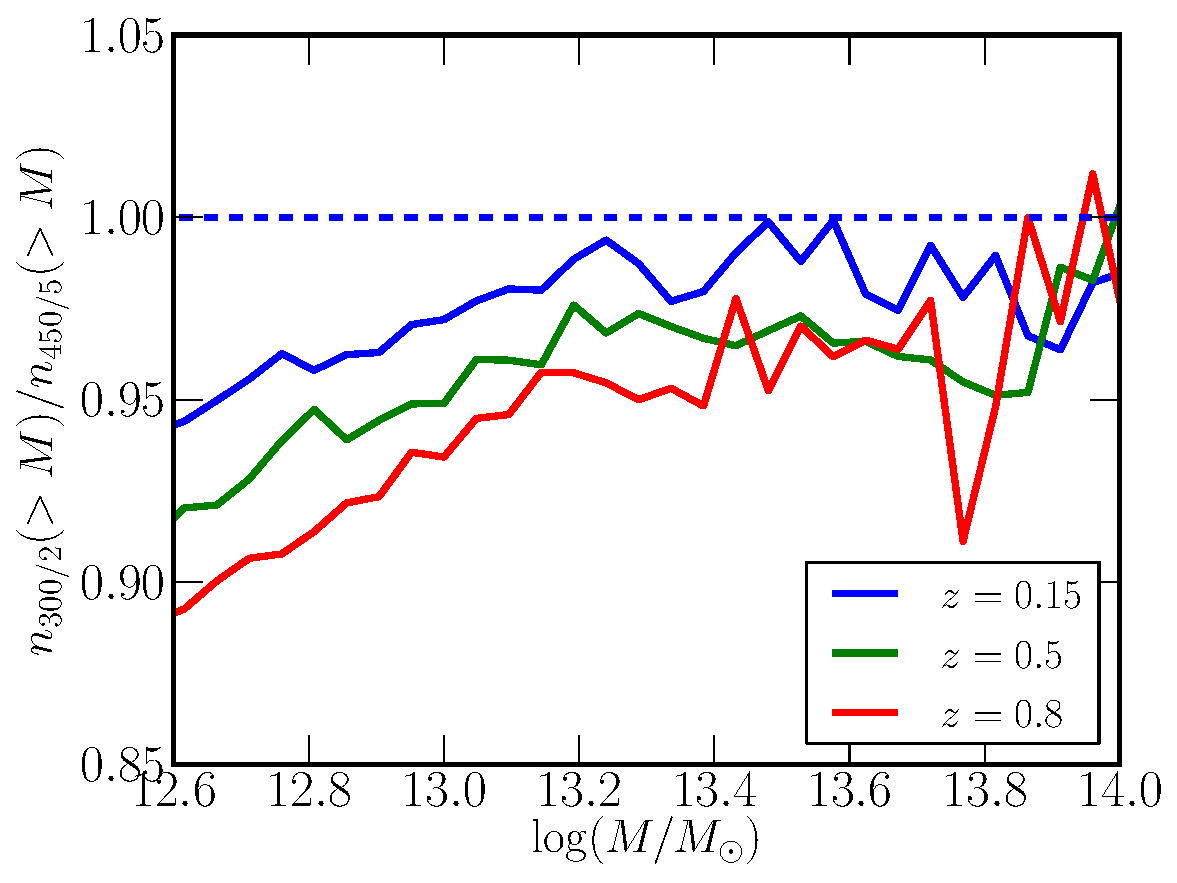
\includegraphics[width=1\columnwidth]{/Users/old_ts485/Dropbox/big-sims/Plots/haloRatioNum_noTweak_redshift}

\caption{\label{fig:massFn_redshift}Comparison of cumulative mass functions
between 450/5 and 300/2 at $z=0.15$, $z=0.5$, and $z=0.8$. For
the larger redshifts, the deviation gets larger particularly on small
halo masses. }


\end{figure}



\subsection{method}

In order to compare halo mass differences between 300/2 and 450/5,
we first match halos in the 300/2 simulation to halos in the 450/5
by using our matching algorithm. Next, we take mean of the halo mass
differences for those matched halos as a function of halo mass of
300/2 and fit the mean to a functional shown below,

\begin{equation}
M_{re}=M_{300/2}(1.0+\alpha(M_{300/2}/10^{12.0}[{\rm M_{\odot}])^{\beta},}
\end{equation}
where $M_{re}$ is a reassigned halo mass for the samples of 300/2,
$M_{300/2}$ is an original halo mass of 300/2, $\alpha$ and $\beta$
are free parameters which are functions of the redshift. By fitting
to the samples of 300/2 to the 450/5 by using the above functional,
we find best fit parameters shown below:

\begin{equation}
\alpha(z)=0.123z+0.052,
\end{equation}
and
\begin{equation}
\beta(z)=-0.154z-0.447.
\end{equation}


Applying the functional to the samples from 300/2, we obtain mass
functions shown in Figure \ref{fig:massFn_tweak}. The match of reassigned
halo mass functions for 300/2 to the 450/5 mass functions is significantly
improved that now the difference is well within 5\% on any halo masses
at any redshifts.

\begin{figure}
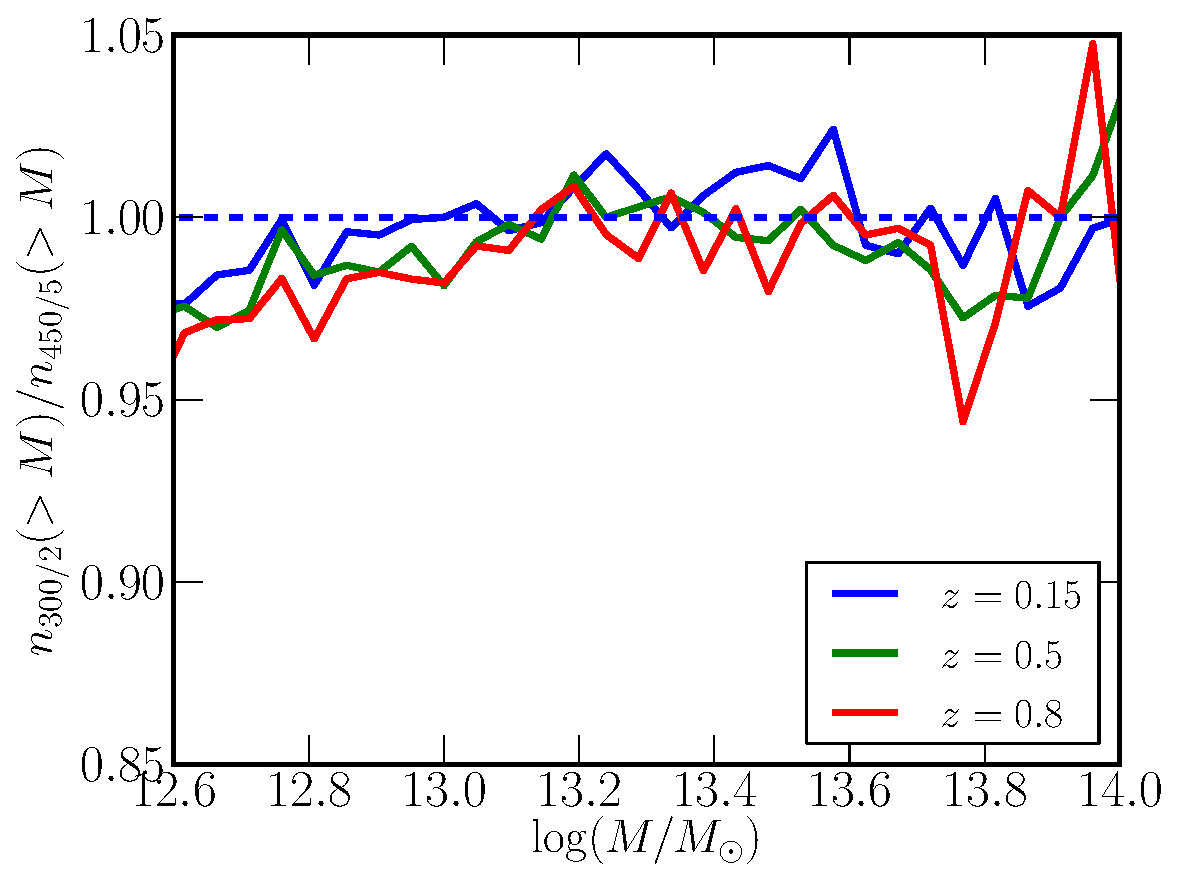
\includegraphics[width=1\columnwidth]{/Users/old_ts485/Dropbox/big-sims/Plots/haloRatioNum_tweak5_redshift}

\caption{\label{fig:massFn_tweak}Comparison of cumulative mass functions after
reassigning halo masses for the simulation of 300/2. The agreement
of 300/2 with 450/5 is significantly improved especially on halo masses
greater than $10^{13.0}{\rm M_{\odot}}$.}
\end{figure}



\subsection{Power Spectra}

We calculate halo-matter cross power spectra after reassigning halo
masses for 300/2, as shown in Figure \ref{fig:crossPower_redshift}.
We use halo mass thresholds of $10^{12.5}{\rm M_{\odot}}$ for the
left panel and $10^{13.0}{\rm M_{\odot}}$ for the right panel. As
expected from the mass functions, the match between 300/2 and 450/5
with the threshold of $10^{13.0}{\rm M_{\odot}}$ is better than the
one with $10^{12.5}{\rm M_{\odot}}$. The agreement between 300/2
and 450/5 is, however, well within 2\% for both cases, which is a
significant improvement compared to the results shown in the previous
section.

\begin{figure}
\includegraphics[width=1\columnwidth]{/Users/old_ts485/Dropbox/Tomomi/HACC/Conv/Matching_halos/20130703/crossMatter_m450_tweak300_2_softMcut13\lyxdot 0_s0\lyxdot 5}

\caption{\label{fig:crossPower_redshift}Ratio of halo-matter cross power spectra
after reassigning halo masses for the sample from the 300/2 simulations.
We select halos based on the soft mass-cut method\textcolor{black}{{}
with $M_{cut}=13.0$ and $\sigma=0.5$. The overall agreements are
well within 2\%.}}


\end{figure}


\begin{table*}[h]
Table: ${\rm log_{10}(M/M_{450/5})}$ 

\begin{tabular}{|c|c|c|c|}
\hline 
z=0.15 & median & $\Delta_{65\%}$ & $\Delta_{95\%}$\tabularnewline
\hline 
\hline 
300/3 & -0.0026 & 0.0877 & 0.2864\tabularnewline
\hline 
300/2 & -0.0078 & 0.0972 & 0.3458\tabularnewline
\hline 
150/3 & -0.0266 & 0.1107  & 0.3101\tabularnewline
\hline 
150/2 & -0.0454 & 0.1207 & 0.3315\tabularnewline
\hline 
\end{tabular}%
\begin{tabular}{|c|c|c|c|}
\hline 
z=0.5 & median & $\Delta_{65\%}$ & $\Delta_{95\%}$\tabularnewline
\hline 
\hline 
300/3 & -0.0062 & 0.0905  & 0.2869\tabularnewline
\hline 
300/2 & -0.0139  & 0.1029 & 0.3345\tabularnewline
\hline 
150/3 & -0.0372  & 0.1148 & 0.3083\tabularnewline
\hline 
150/2 & -0.0595 & 0.1252 & 0.3093\tabularnewline
\hline 
\end{tabular}%
\begin{tabular}{|c|c|c|c|}
\hline 
z=0.8 & median & $\Delta_{65\%}$ & $\Delta_{95\%}$\tabularnewline
\hline 
\hline 
300/3 & -0.0067 & 0.0932 & 0.2891\tabularnewline
\hline 
300/2 & -0.0189  & 0.1048  & 0.3347\tabularnewline
\hline 
150/3 & -0.0519 & 0.1172 & 0.2926\tabularnewline
\hline 
150/2 & -0.0782 & 0.1274 & 0.28878\tabularnewline
\hline 
\end{tabular}

\caption{\label{tab:HaloMass}Comparison of halo mass ratios ${\rm log_{10}M/M_{450/5}}$
in log-based, comparing various time steps to the 450/5 simulation
at $z=0.15$, $z=0.5$, and $z=0.8$. For each redshift, we report
median, $\Delta_{95\%}$, and $\Delta_{65\%}$ (how should I explain
about $\Delta_{95\%}$?). As shown in Figure \ref{fig:HaloProperty_step},
the results indicate that mass ratio distributions for the 300 global
steps have less scatter than for the 150 global steps.}
\end{table*}


\begin{table*}[H]
\begin{tabular}{|c|c|c|c|}
\hline 
z=0.15 & median & $\Delta_{65\%}$ & $\Delta_{95\%}$\tabularnewline
\hline 
\hline 
${\rm M_{halo}\in[10^{12.5},10^{13.0}]}$ & -0.0111 & 0.1124 & 0.3896\tabularnewline
\hline 
${\rm M_{halo}\in[10^{13.0},10^{13.5}]}$ & -0.0085 & 0.0748 & 0.2599\tabularnewline
\hline 
${\rm M_{halo}\in[10^{13.5},10^{14.0}]}$ & -0.0056 & 0.0471 & 0.1596\tabularnewline
\hline 
${\rm M_{halo}>10^{14.0}}$ & -0.0047 & 0.0341 & 0.1323\tabularnewline
\hline 
\end{tabular}%
\begin{tabular}{|c|c|c|c|}
\hline 
z=0.5 & median & $\Delta_{65\%}$ & $\Delta_{95\%}$\tabularnewline
\hline 
\hline 
${\rm M_{halo}\in[10^{12.5},10^{13.0}]}$ & -0.0197 & 0.1156 & 0.3544\tabularnewline
\hline 
${\rm M_{halo}\in[10^{13.0},10^{13.5}]}$ & -0.0123 & 0.0790 & 0.2546\tabularnewline
\hline 
${\rm M_{halo}\in[10^{13.5},10^{14.0}]}$ & -0.0067 & 0.0497 & 0.1813\tabularnewline
\hline 
${\rm M_{halo}>10^{14.0}}$ & -0.0052 & 0.0309 & 0.0731\tabularnewline
\hline 
\end{tabular}%
\begin{tabular}{|c|c|c|c|}
\hline 
z=0.8 & median & $\Delta_{65\%}$ & $\Delta_{95\%}$\tabularnewline
\hline 
\hline 
${\rm M_{halo}\in[10^{12.5},10^{13.0}]}$ & -0.0260 & 0.1161 & 0.3478\tabularnewline
\hline 
${\rm M_{halo}\in[10^{13.0},10^{13.5}]}$ & -0.0167 & 0.0835 & 0.2546\tabularnewline
\hline 
${\rm M_{halo}\in[10^{13.5},10^{14.0}]}$ & -0.0084 & 0.0490 & 0.1809\tabularnewline
\hline 
${\rm M_{halo}>10^{14.0}}$ & -0.0077 & 0.0297 & 0.1361\tabularnewline
\hline 
\end{tabular}

\caption{\label{tab:HaloMassSlice}Comparison of halo mass ratios ${\rm log_{10}M_{300/2}/M_{450/5}}$
in log-based, comparing the 300/2 to the 450/5 simulation as a function
of halo mass slices at $z=0.15$, $z=0.5$, and $z=0.8$. For each
redshift, we report median, $\Delta_{95\%}$, and $\Delta_{65\%}$.
As shown, medians and $\Delta$s decreases as increasing halo mass
and decreasing redshift.}
\end{table*}


\begin{table*}[H]
\begin{tabular}{|c|c|c|c|}
\hline 
z=0.15 & median & $\Delta_{65\%}$ & $\Delta_{95\%}$\tabularnewline
\hline 
\hline 
300/3 & 0.1116 & 0.1228 & 0.4439\tabularnewline
\hline 
300/2 & 0.1245 & 0.1406 & 0.5558\tabularnewline
\hline 
150/3 & 0.2706 & 0.2571 & 0.6234\tabularnewline
\hline 
150/2 & 0.2800 & 0.2680 & 0.6568\tabularnewline
\hline 
\end{tabular}%
\begin{tabular}{|c|c|c|c|}
\hline 
z=0.5 & median & $\Delta_{65\%}$ & $\Delta_{95\%}$\tabularnewline
\hline 
\hline 
300/3 & 0.1221 & 0.1298 & 0.4700\tabularnewline
\hline 
300/2 & 0.1348 & 0.1460 & 0.5400\tabularnewline
\hline 
150/3 & 0.2382 & 0.2248 & 0.5555\tabularnewline
\hline 
150/2 & 0.2475 & 0.2335 & 0.5835\tabularnewline
\hline 
\end{tabular}%
\begin{tabular}{|c|c|c|c|}
\hline 
z=0.8 & median & $\Delta_{65\%}$ & $\Delta_{95\%}$\tabularnewline
\hline 
\hline 
300/3 & 0.1217 & 0.1329 & 0.4553\tabularnewline
\hline 
300/2 & 0.1354 & 0.1498 & 0.4969\tabularnewline
\hline 
150/3 & 0.2447 & 0.2284 & 0.5408\tabularnewline
\hline 
150/2 & 0.2536 & 0.2334 & 0.5418\tabularnewline
\hline 
\end{tabular}

\caption{\label{tab:HaloPosition}Comparison of halo positions for various
time steps to the 450/5 simulation at $z=0.15$, $z=0.5$, and $z=0.8$.
For each redshift, we report median, $\Delta_{95\%}$, and $\Delta_{65\%}$.
As shown, the halo positions for the 150 global steps are more scattered
and 3 and 2 sub-cycles affect negligibly on halo positions. Also,
there is little change due to redshift.}
\end{table*}
 

\begin{table*}
\begin{tabular}{|c|c|c|c|}
\hline 
z=0.15 & median & $\Delta_{65\%}$ & $\Delta_{95\%}$\tabularnewline
\hline 
\hline 
300/3 & -3.36 & 24.3872 & 82.20\tabularnewline
\hline 
300/2 & -3.26 & 27.5063 & 99.40\tabularnewline
\hline 
150/3 & -16.61 & 38.4702 & 116.93\tabularnewline
\hline 
150/2 & -17.05  & 39.9572 & 121.45 \tabularnewline
\hline 
\end{tabular}%
\begin{tabular}{|c|c|c|c|}
\hline 
z=0.5 & median & $\Delta_{65\%}$ & $\Delta_{95\%}$\tabularnewline
\hline 
\hline 
300/3 & -3.78 & 36.87 & 118.48\tabularnewline
\hline 
300/2 & -3.94 & 40.77 & 137.62 \tabularnewline
\hline 
150/3 & -23.25  & 53.41  & 151.75 \tabularnewline
\hline 
150/2 & -24.26 & 56.75 & 160.15 \tabularnewline
\hline 
\end{tabular}%
\begin{tabular}{|c|c|c|c|}
\hline 
z=0.8 & median & $\Delta_{65\%}$ & $\Delta_{95\%}$\tabularnewline
\hline 
\hline 
300/3 & -6.32 & 47.41 & 149.72\tabularnewline
\hline 
300/2 & -6.47  & 53.48  & 169.1556\tabularnewline
\hline 
150/3 & -25.23 & 67.62 & 186.29\tabularnewline
\hline 
150/2 & -24.76 &  71.97 &  189.26\tabularnewline
\hline 
\end{tabular}

\caption{\label{tab:HaloVelocity}Comparison of halo velocity for various time
steps to the 450/5 simulation at $z=0.15$, $z=0.5$, and $z=0.8$.
For each redshift, we report median, $\Delta_{95\%}$, and $\Delta_{65\%}$.
As shown in Figure \ref{fig:HaloProperty_step}, the results indicate
that mass ratio distributions for the 300 global steps have less scatter
than for the 150 global steps.}
\end{table*}
 
\begin{table*}
\begin{tabular}{|c|c|}
\hline 
z=0.15 & fraction within 10 degree\tabularnewline
\hline 
\hline 
300/3 & 0.951\tabularnewline
\hline 
300/2 & 0.938\tabularnewline
\hline 
150/3 & 0.928\tabularnewline
\hline 
150/2 & 0.923\tabularnewline
\hline 
\end{tabular}

\caption{\label{tab:HaloVelPhase}Fractions of halos whose velocity direction
matches with the 450/5 within 10 degree at $z=0.15$. More than 90\%
f halos for any time steps agree with the 450/5 simulation.}
\end{table*}

\end{document}
